%! TeX program = lualatex
\documentclass[a4paper]{article} 

% packages
\usepackage{microtype}      % Slightly tweak font spacing for aesthetics
\usepackage[english]{babel} % Language hyphenation and typographical rules
\usepackage[final, colorlinks = false, urlcolor = cyan]{hyperref} 
\usepackage{changepage}     % adjust margins on the fly
\usepackage{fontspec}

\usepackage{minted}
% \usemintedstyle{algol_nu}
\usepackage{xcolor}

\usepackage{pgfplots}
\pgfplotsset{width=\textwidth,compat=1.9}

\usepackage{caption}
\newenvironment{code}{\captionsetup{type=listing}}{}
\captionsetup[listing]{skip=0pt}
\setlength{\abovecaptionskip}{5pt}
\setlength{\belowcaptionskip}{5pt}

\usepackage[yyyymmdd]{datetime}
\renewcommand{\dateseparator}{--}
\setmainfont{EB Garamond}
\setmonofont[Scale=MatchLowercase]{Deja Vu Sans Mono}

\usepackage{titlesec}
% \titleformat{\section}{\LARGE\bfseries}{}{}{}[\titlerule]
% \titleformat{\subsection}{\Large\bfseries}{}{0em}{}
% \titlespacing{\subsection}{0em}{-0.7em}{0em}
%
% \titleformat{\subsubsection}{\large\bfseries}{}{0em}{$\bullet$ }
% \titlespacing{\subsubsection}{1em}{-0.7em}{0em}

% margins
\addtolength{\hoffset}{-2.25cm}
\addtolength{\textwidth}{4.5cm}
\addtolength{\voffset}{-3.25cm}
\addtolength{\textheight}{5cm}
\setlength{\parskip}{0pt}
\setlength{\parindent}{0in}
% \setcounter{secnumdepth}{0}

\begin{document}
\hrule \medskip
\begin{minipage}{0.295\textwidth} 
    \raggedright
    \footnotesize 
    Name: Andrew Hayes \\
    E-mail: \href{mailto://a.hayes18@universityofgalway.ie}{\texttt{a.hayes18@universityofgalway.ie}}  \hfill\\   
    ID: 21321503 \hfill
\end{minipage}
\begin{minipage}{0.4\textwidth} 
    \centering 
    \vspace{0.4em}
    \Large 
    \textbf{CT331} \\ 
\end{minipage}
\begin{minipage}{0.295\textwidth} 
    \raggedleft
    \today
\end{minipage}
\medskip\hrule 
\begin{center}
    \normalsize
    Assignment 3: Declarative Programming with Prolog
\end{center}
\hrule

\section{Question 1}
\subsection{Rule that returns true if a given instructor teaches a given student}
\begin{minted}[linenos, breaklines, frame=single]{prolog}
teaches(Instructor, Student) :- instructs(Instructor, Course), takes(Student, Course).
\end{minted}

\subsection{Query that uses the \mintinline{prolog}{teaches} rule to show all students instructed by \mintinline{prolog}{bob}}
For this, I wasn't sure if the desired answer was a query that returned a student instructed by \mintinline{prolog}{bob}, followed by 
a couple semi-colons to get every student instructed by \mintinline{prolog}{bob}, or if the desired answer was a single query that 
returned a list of students taught by \mintinline{prolog}{bob}, so I did both.
\begin{minted}[linenos, breaklines, frame=single]{prolog}
?- teaches(bob, Student).
\end{minted}

\begin{figure}[H]
    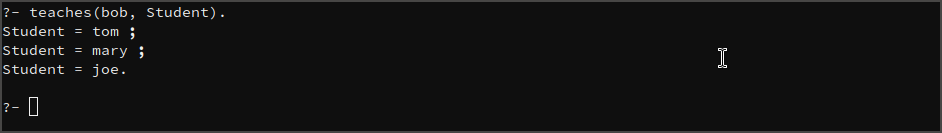
\includegraphics[width=\textwidth]{./images/q1.2.png}
    \caption{Using the \mintinline{prolog}{teaches} rule to show all students instructed by \mintinline{prolog}{bob}}
\end{figure}

Alternatively, this could be done using the \mintinline{prolog}{findall()} predicate:
\begin{minted}[linenos, breaklines, frame=single]{prolog}
?- findall(Student, teaches(bob, Student), Students).
\end{minted}

\begin{figure}[H]
    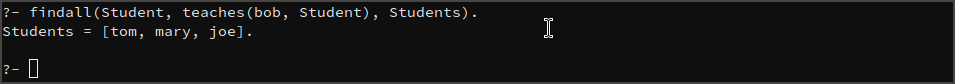
\includegraphics[width=\textwidth]{./images/q1_2_findall.png}
    \caption{Using the \mintinline{prolog}{teaches} rule \& the \mintinline{prolog}{findall} predicate to show all students instructed by \mintinline{prolog}{bob}}
\end{figure}

\subsection{Query that uses the \mintinline{prolog}{teaches} rule to show all instructors that instruct \mintinline{prolog}{mary}}
\begin{minted}[linenos, breaklines, frame=single]{prolog}
?- teaches(Instructor, mary).
\end{minted}

\begin{figure}[H]
    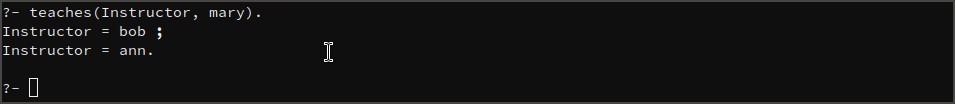
\includegraphics[width=\textwidth]{./images/q1_3.png}
    \caption{Using the \mintinline{prolog}{teaches} rule to show all instructors that instruct \mintinline{prolog}{mary}}
\end{figure}

Alternatively, this could be done using the \mintinline{prolog}{findall()} predicate:
\begin{minted}[linenos, breaklines, frame=single]{prolog}
?- findall(Instructor, teaches(Instructor, mary), Instructors).
\end{minted}

\begin{figure}[H]
    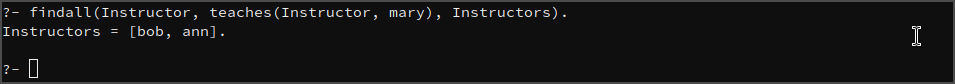
\includegraphics[width=\textwidth]{./images/q1_3_findall.png}
    \caption{Using the \mintinline{prolog}{teaches()} rule \& the \mintinline{prolog}{findall()} predicate to show all instructors that instruct \mintinline{prolog}{mary}}
\end{figure}

\subsection{Result of query \mintinline{prolog}{teaches(ann,joe).}}
\begin{figure}[H]
    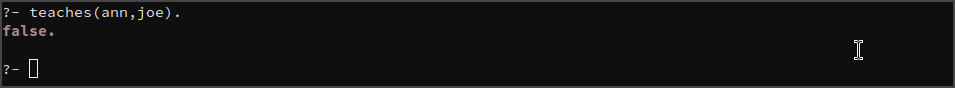
\includegraphics[width=\textwidth]{./images/q1_4.png}
    \caption{Result of query \mintinline{prolog}{teaches(ann,joe).}}
\end{figure}

The result of the query \mintinline{prolog}{teaches(ann,joe).} is \mintinline{prolog}{false.} because \mintinline{prolog}{ann}
only instructs \mintinline{prolog}{ct345} and \mintinline{prolog}{joe} only takes \mintinline{prolog}{ct331}, and therefore 
\mintinline{prolog}{ann} does not teach \mintinline{prolog}{joe} because \mintinline{prolog}{ann} does not teach a course
that \mintinline{prolog}{joe} takes.

\subsection{Rule that returns \mintinline{prolog}{true} if two students take the same course}
\begin{minted}[linenos, breaklines, frame=single]{prolog}
takesSameCourse(Student1, Student2) :- takes(Student1, Course), takes(Student2, Course).
\end{minted}

\begin{figure}[H]
    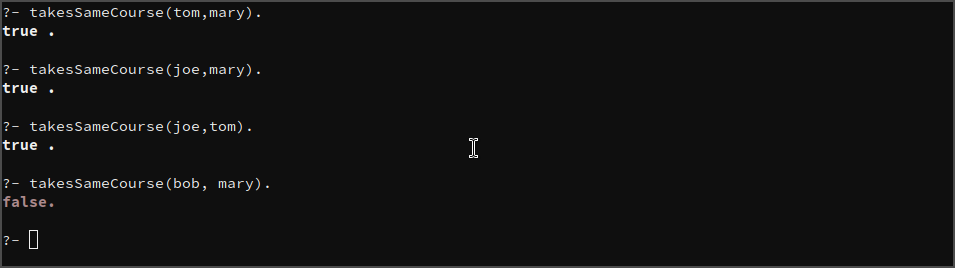
\includegraphics[width=\textwidth]{./images/q1_5.png}
    \caption{Queries to test \mintinline{prolog}{takesSameCourse()}}
\end{figure}

\begin{minted}[linenos, breaklines, frame=single]{prolog}
?- takesSameCourse(tom,mary).
?- takesSameCourse(joe,mary).
?- takesSameCourse(joe,tom).
?- takesSameCourse(bob, mary).
\end{minted}

\section{Question 2}
\subsection{Query that displays the head \& tail of a list}
\begin{minted}[linenos, breaklines, frame=single]{prolog}
?- [Head | Tail] = [1,2,3].
\end{minted}

\begin{figure}[H]
    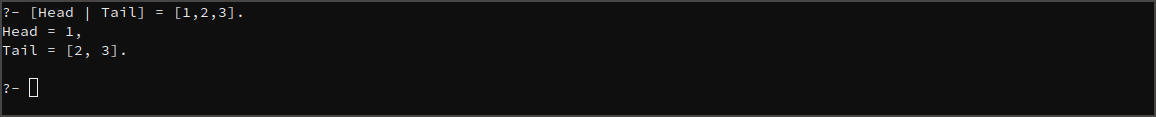
\includegraphics[width=\textwidth]{./images/q2_1.png}
    \caption{Query to display the head \& tail of the list \mintinline{prolog}{[1,2,3]}}
\end{figure}

\subsection{Display the head of a list, the head of the tail of the list, \& the tail of the tail of the list}
\begin{minted}[linenos, breaklines, frame=single]{prolog}
?- [Head | [HeadOfTail | TailOfTail]] = [1,2,3,4,5].
\end{minted}

\begin{figure}[H]
    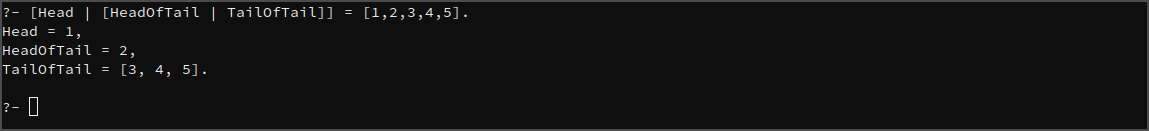
\includegraphics[width=\textwidth]{./images/q2_2.png}
    \caption{Query to display the head of the list, the head of the tail of the list, \& the tail of the tail of the list \mintinline{prolog}{[1,2,3,4,5]}}
\end{figure}

\subsection{Rule that returns \mintinline{prolog}{true} if a given element is the first element of a given list}
\begin{minted}[linenos, breaklines, frame=single]{prolog}
contains1(Element, [Element | Tail]).

?- contains1(1, [1,2,3,4]).
?- contains1(3, [1,2,3,4]).
?- contains1(1, [2,3,4]).
\end{minted}

\begin{figure}[H]
    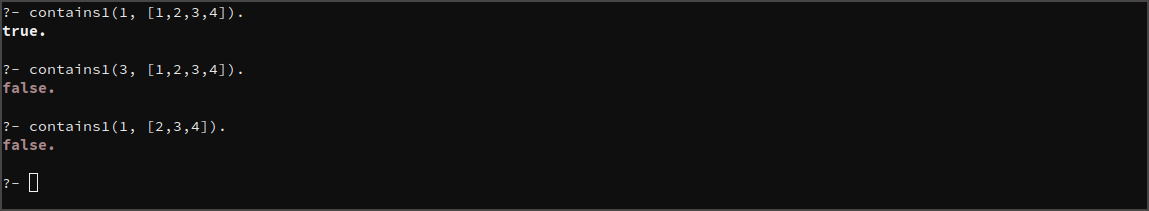
\includegraphics[width=\textwidth]{./images/q2_3.png}
    \caption{\mintinline{prolog}{contains1()} testing}
\end{figure}

\subsection{Rule that returns \mintinline{prolog}{true} if a given list is the same as the tail of another given list}
\begin{minted}[linenos, breaklines, frame=single]{prolog}
contains2(Sublist, [Head | Sublist]).

?- contains2([2,3,4], [1,2,3,4]).
?- contains2([2,3,4], [1,2,3,4,5]).
\end{minted}

\begin{figure}[H]
    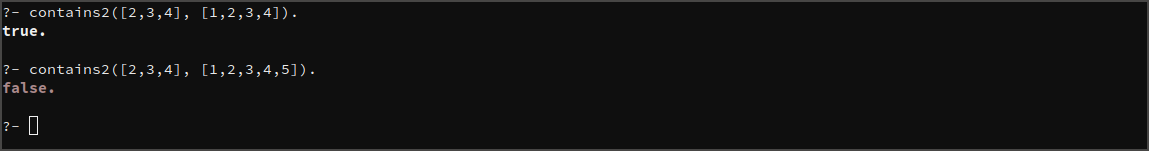
\includegraphics[width=\textwidth]{./images/q2_4.png}
    \caption{\mintinline{prolog}{contains2()} testing}
\end{figure}

\subsection{Query to display the first element of a given list using \mintinline{prolog}{contains1()}}
\begin{minted}[linenos, breaklines, frame=single]{prolog}
?- contains1(FirstElement, [1,2,3,4,5]).
\end{minted}

\begin{figure}[H]
    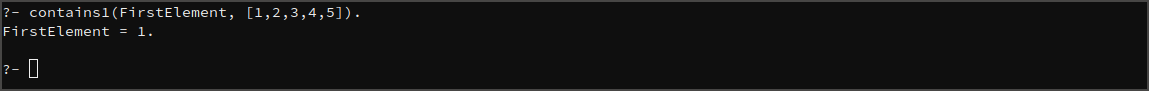
\includegraphics[width=\textwidth]{./images/q2_5.png}
    \caption{Query to display the first element of a given list using \mintinline{prolog}{contains1()}}
\end{figure}

\section{Determine if a given element is not in a given list}
\begin{minted}[linenos, breaklines, frame=single]{prolog}
% base case: any element is not in an empty list
isNotElementInList(_, []).

% return true if Element is not the Head of the list and it's not found recursively searching the rest of the list
isNotElementInList(Element, [Head | Tail]) :- Element \= Head, isNotElementInList(Element, Tail).

% testing
isNotElementInList(1, []).  
isNotElementInList(1, [1]). 
isNotElementInList(1, [2]).  
isNotElementInList(2, [1, 2, 3]).  
isNotElementInList(7, [1, 2, 9, 4, 5]). 
\end{minted}

\begin{figure}[H]
    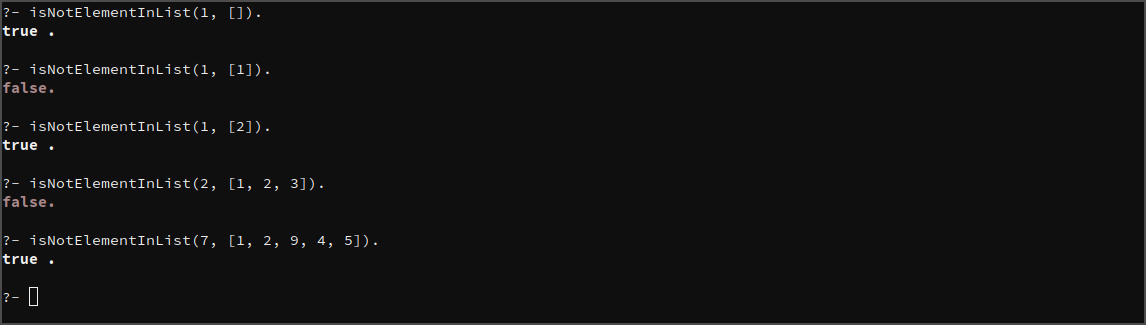
\includegraphics[width=\textwidth]{./images/q3.png}
    \caption{Testing \mintinline{prolog}{isNotElementInList()}}
\end{figure}

\section{Facts \& rules to merge three lists}
\begin{minted}[linenos, breaklines, frame=single]{prolog}
% predicate to merge two lists
% base case: if the first list is empty, just return the second
mergeTwoLists([], List, List).

% recursive predicate to merge two lists
% split the first list into head and tail, and recurse with its tail and the second list until the first list is empty (base case)
% then merge the original head of the first list with the resulting tail
mergeTwoLists([Head | Tail], List2, [Head | ResultTail]) :- mergeTwoLists(Tail, List2, ResultTail).

% predicate to merge 3 lists 
% base case: merging an empty list and two others is the same as merging two lists
mergeLists([], List2, List3, Merged) :- mergeTwoLists(List2, List3, Merged).

% split the first list into head and tail, and recurse with its tail and the other two lists until the first list is empty (base case)
mergeLists([Head1 | Tail1], List2, List3, [Head1 | MergedTail]) :- mergeLists(Tail1, List2, List3, MergedTail).

?- mergeLists([7],[1,2,3],[6,7,8], X).
?- mergeLists([2], [1], [0], X).
?- mergeLists([1], [], [], X).
\end{minted}

\begin{figure}[H]
    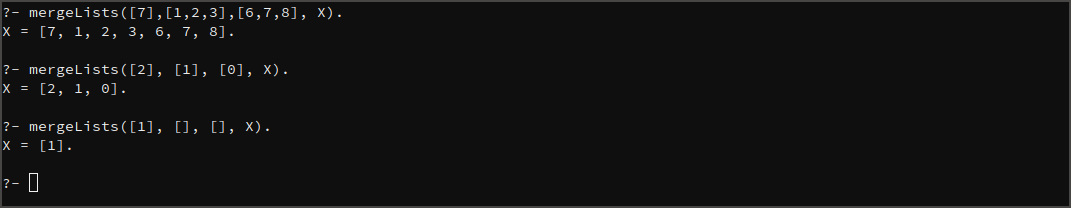
\includegraphics[width=\textwidth]{./images/q4.png}
    \caption{Testing \mintinline{prolog}{mergeLists()}}
\end{figure}

\section{Facts \& rules to reverse a given list}
\begin{minted}[linenos, breaklines, frame=single]{prolog}
% call the helper predicate with the list to be reversed and an empty Accumulator to build up
reverseList(List, Reversed) :- reverseListHelper(List, [], Reversed).

% base case fact: when the list to reverse is empty, the accumulator is the reversed list
reverseListHelper([], Accumulator, Accumulator).

% recurse with the tail after prepending the head to the accumulator
reverseListHelper([Head | Tail], Accumulator, Reversed) :- reverseListHelper(Tail, [Head | Accumulator], Reversed).

?- reverseList([1,2,3], X).  
?- reverseList([1], X).  
?- reverseList([], X).  
\end{minted}

\begin{figure}[H]
    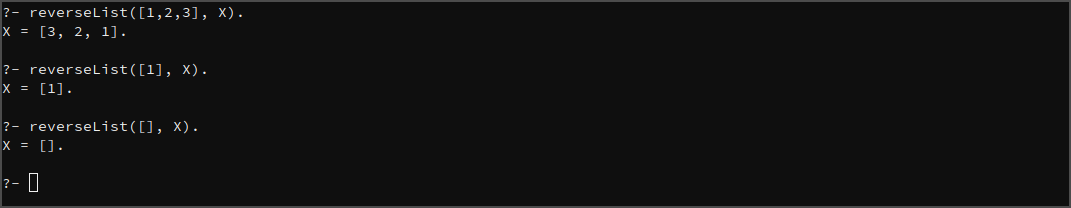
\includegraphics[width=\textwidth]{./images/q5.png}
    \caption{Testing \mintinline{prolog}{reverseList()}}
\end{figure}

\section{Facts \& rules to insert an element into its correct position in a given list}
\begin{minted}[linenos, breaklines, frame=single]{prolog}
% base fact: if the list is empty, the list to be returned is just the element
insertInOrder(Element, [], [Element]).

% if the element to be inserted is <= the head of the list, insert it at the head of the list
insertInOrder(Element, [Head | Tail], [Element, Head | Tail]) :- Element =< Head.

% if the element to be inserted is greater than the head of the list, recurse with the tail of the list until 
insertInOrder(Element, [Head | Tail], [Head | NewTail]) :- Element > Head, insertInOrder(Element, Tail, NewTail).
\end{minted}

\begin{figure}[H]
    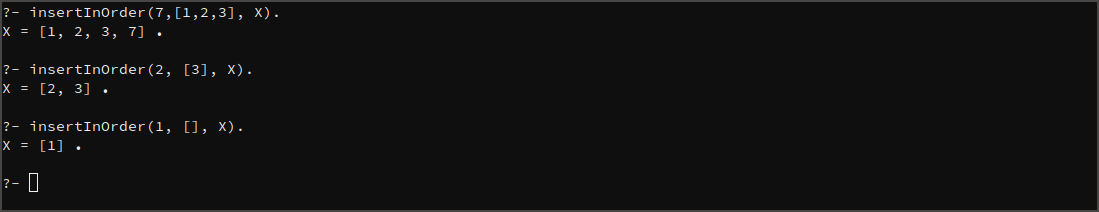
\includegraphics[width=\textwidth]{./images/q6.png}
    \caption{Testing \mintinline{prolog}{insertInOrder()}}
\end{figure}


\end{document}
